\chapter{Fundamentos y Estado del arte}

%En este capítulo se intentara dar una breve reseña de las investigaciones mas recientes en el campo de las comunicaciones ópticas. 
En este capítulo se presentan las bases y fundamentos de las técnicas desarrolladas y utilizadas en esta tésis. 
Primeramente se da una breve explicación de los conceptos de códigos correctores de errores, continuando con los distintos algoritmos utilizados en la implementación. Luego, se explicará el concepto de espectro ensanchado, una técnica utilizada en comunicaciones pero implementada de un modo poco convencional en este trabajo. Posteriormente se repasarán los aspectos de seguridad a tener en cuenta al utilizar los algoritmos previamente mencionados, los conceptos de niveles de fuerza criptográficas y de cual es el objetivo a alcanzar con respecto a este último tema.

Para finalizar, en la sección de estado del arte se repasarán el estado de las tecnologías y sistemas en uso actualmente, a modo de comparación con el descrito en esta tesis.

\section{Códigos correctores de errores}

Para trasmitir información digital a través de un medio analógico tal como una fibra óptica, deben convertirse las señales digitales original a señales analógicas.
Toda señal analógica que se transmite o almacen en algún medio físico invariablemente se sufre una degradación, producto de las imperfecciones de los transductores, imperfecciones o limitaciones en la codificación o ruido de diferentes tipos. Esta degradación puede ocurrir en cualquier módulo del sistema, o las interfaces entre los mismos, y generalmente es deseable que el sistema pueda reproducir los datos almacenados o transmitidos con la menor cantidad posible de errores. La diferencia entre la señal transmitida y la recibida se suele modelar como una señal de ruido con una determinada distribución de potencia superpuesta a la señal codificada. Algunos modelos de ruido son muy utilizados, tal como el ruido aditivo gaussiano, utilizado para modelar la interferencia producto de fuentes naturales como ruido térmico o para aproximar fuentes de ruido no-lineales.

Al transmitir datos digitales sobre canales con ruido, aún asumiendo que las etapas moduladoras y demoduladoras son capaces de reproducir los datos fielmente, el mensaje recibido $m_r$ sera distinto del mensaje original $m$, ya que la señal que recibe el demodulador sera una combinación de la señal original del demodulador con el ruido. La diferencia entre la señal recibida $m_r$ y $m$ se denomina error de transmisión. Para aumentar la confiabilidad y reducir el error de transmisión se idearon códigos correctores/detectores de errores, con los que el receptor puede detectar un error y pedir una retransmisión, o bien corregir el error utilizando datos adicionales presentes en la señal. Los métodos de corrección de errores generalmente funcionan reduciendo la entropía de la información transmitida, aumentando la redundancia de la información.

Un método trivial de corrección de errores consiste en utilizar un código de detección de errores como puede ser una suma de verificación, el algoritmo CRC o función de hash \cite{Menezes:1996:HAC:548089}, e iniciar un proceso de retransmisión del segmento o trama de datos afectada. Esté simple método posee la desventaja de ser costoso tanto en ancho de banda utilizado, como en el retraso de la transmisión. En enlaces de muy alta velocidad, las elevadas tasas de retransmisiones hacen a este algoritmo sumamente ineficiente.

Por lo tanto es deseable utilizar un algoritmo que pueda detectar y corregir errores basado solamente en información adicional transmitida, sin utilizar retransmisiones. Esta técnica se denomina \textsl{Forward Error Correction Codes}, o códigos FEC \cite{Moon:05} de los cuales existen diferentes tipos de acuerdo con sus aplicación, performance y parámetros. A continuación, se describen los algoritmos que fueron utilizados en el sistema propuesto en esta tesis.

\subsection{BCH/Reed Solomon}
Los códigos BCH y Reed-Solomon~\cite{reed1960polynomial} son usados ampliamente en la industria de comunicaciones y almacenamiento masivo ya que la implementación es eficientes desde el punto de vista del radio entre errores corregidos e información de paridad agregada. De echo, Reed-Solomon pertenece a una clase de códigos lineales denominados MDS (\textit{maximum distance separable}) que se consideran óptimos en esta relación. Estos códigos consisten en una representación de los datos basada en grupos algebraicos cíclicos. 
Esta familia de códigos fue introducida en 1959, pero es todavía utilizada en estándares de Ethernet de 10Gbps, 100Gbps y hasta 400Gbps~\cite{liforward} debido a su robustez, bajo retraso y la existencia de algoritmos eficientes para la decodificación en un tiempo fijo.

\subsection{LDPC}
El esquema de corrección de errores LDPC~\cite{gallagerpress} (\textit{Low Density Parity Check}, también conocidos como códigos de Gallager) es un caso notable. Introducido en los años 60, fue olvidado debido a la alta capacidad de procesamiento y memoria requerido por el mismo, ya que para su implementación es necesario utilizar matrices de paridad de un tamaño elevado. Sin embargo, con los modernos avances en hardware informático, éste algoritmo se volvió una opción viable y actualmente es utilizado en sistemas modernos~\cite{brack2007low} debido a su simplicidad y gran capacidad de corrección de errores, en algunos casos muy cercana a la máxima capacidad teórica del canal.
Antes de ahondar en la descripción de este algoritmo debemos aclarar que, a pesar de ser utilizado para ciertos modelos durante la primera fase de la investigación, fue descartado en la versión final por un modelo mas simple y con menos requerimientos de hardware que presenta una desempeño similar desde el punto de vista de corrección de errores.

LDPC es un código que se denomina ``\textit{capacity-approaching}'' o sea, que para un canal discreto sin memoria, el ruido del mismo puede ser estar muy cerca del límite teórico de Shannon~\cite{shannon48}.
El algoritmo se basa en un código lineal que utiliza una matriz de paridad $H$ grande y dispersa. Esta matriz tiene la propiedad de que todo codeword $x$ válido cumple con $H*x=0$. 
Existen muchos métodos para construir la matriz de paridad; uno muy utilizado consiste simplemente en generarla aleatoriamente. Otras maneras de generar la matriz son posibles y es un campo de investigación activo actualmente.

% Meter en apendice
%\paragraph{LDPC: Generador de matriz}
%La matriz generadora puede crearse fácilmente si H es de la forma $[D|I]$, simplemente formando la matriz:
%$$G=[I|D']$$
%Donde D' es la transpuesta de la matriz D
%Para la generación de la matriz se opto por utilizar un algoritmo aleatorio y luego aplicando testeos de validación, para lograr una matriz sistemática de rate entero (1/2, 1/3, etc.)
%Para verificar se G genera vectores cuya matriz de paridad es H, puede verificarse que:
%$$ H*G'=0 $$

%Podemos definir la matriz de paridad $H$ como una matriz de paridad que tenga mas de 3 unos por fila y una cantidad similar por columna. Buenos resultados se obtienen a partir de matrices de 200x100.
%Se puede comenzar por una matriz vacía $H = 0$ del tamaño deseado, y ir agregándole unos al azar. Cierto análisis es necesario para garantizar que no se cumplan ciclos y que la cantidad de unos por columna y por fila es la deseada. De esto se encargan los algoritmos llamados evencol y evenrow.

%El generador puede generar matrices de cualquier tamaño, de esta manera:

%$$ ./genMatrix <width> <height> <ones per row>$$

%La matriz se genera en la salida estándar. El formato es el utilizado por la biblioteca boost:ublas [CITA].

%NOTA: La matriz siempre esta compuesta de símbolos en GF(2) (O sea, ceros y unos)

%\paragraph{LDPC: encoder}

%El vector inicial se toma de la entrada estándar (stdin) y el codeword se emite en la salida estándar (stdout). La sintaxis es muy sencilla:

%$$ ./ldpcen <matriz> < in >out $$
%\paragraph{LDPC: decoder}
%Si se invoca este filtro mediante el nombre decodificador, tomara el codeword de la entrada estandard, aplicara el algoritmo de belief-propagation (Hard-decision) y se emite el vector original por la salida estandard:
%La diferencia radica que en nuestro caso, al ser un canal asimetrico no se permite el bit-flip de un valor cero a un valor uno, ya que es imposible que se produzca ese error.
%La linea de comando es la siguiente:

%$$ ./ldpcdec <matriz> <in >out $$

%La conversión codeword->vector es sencilla, ya que al ser un código sistemático solo se necesita eliminar la parte del vector que representa la paridad añadida.

%Se generaron muchas matrices, desde 256x128 hasta matrices muy grandes de 10000x5000, pero el tiempo de decodificación crece enormemente para matrices grandes.

%\paragraph{LDPC: optimización}

%Debido a la naturaleza iterativa del decodificador LDPC, pronto se convirtió en el cuello de botella de la simulación. Para acelerar el sistema, se opto por realizar la siguiente optimización:
%Desde el punto de vista algorítmico, LDPC consta básicamente de varios loops, dentro de los cuales se accede a la matriz de paridad, y a otras matrices que acumulan datos intermedios. Primeramente la implementación fue realizada como mencionamos utilizando boost:ublas, pero luego se comprobó que una implementación utilizando arrays de C era hasta 3 veces mas rápida.
%Luego se procedió a realizar un algoritmo de ``unrolling'' de estos loops, generando código especifico a una matriz dada, sin ningún tipo de loop. Obviamente este código es mucho mas grande, pero la aceleración provista es aun mayor, del orden de 8 veces mas rápido que en implementaciones iniciales.
%La manera de invocar el generador de código es la siguiente:

%$$ ./genLdpcDecoder matriz  > decodeGen.h $$

%El archivo generado decodeGen.h es el decodificador especifico para la matriz dada. Este encabezado de C es luego incluido desde el decodificador ldpcenc.cpp y compilado. Al ser generalmente un archivo de un megabyte para una matriz pequeña de 1024x512, el proceso de compilación el largo y requiere de mucha memoria.
%Por otra parte, no se optimizo el proceso de codificación LDPC, ya que consiste solo de una multiplicación de un vector por una matriz, y es una de las tareas en la que boost:ublas es especialmente eficiente.

%\subsubsection{Viterbi/Convolucional}

\section{CDMA}
\label{espectroensanchado}
La multiplexación por división de código, acceso múltiple por división de código o CDMA (del inglés \textit{Code Division Multiple Access}) es el nombre genérico de varias técnicas de comunicación basadas en el espectro expandido, con el fin de lograr multiplexación o control de acceso al medio. 
Se denomina espectro expandido a la utilización de mayor ancho de banda que el necesario para la transmisión correcta de los datos. Generalmente se logra mediante la combinación de una señal señal de ensanchamiento o de pseudo-ruido, con la señal original, utilizando diferentes métodos.

Los orígenes datan del 1903, cuando Nicola Tesla patentó el concepto de \textit{Frequency hopping} o salto en frecuencia, uno de los métodos de CDMA utilizados actualmente.

Estas técnicas apuntan a agregar las siguientes propiedades en el sistema de comunicaciones:
\begin{enumerate} 
\item Resistencia contra ruido e interferencias: ya que el ruido solo afecta una parte del espectro, ante la presencia de ruido, la mayoría de la señal no se verá afectada, pudiéndose recuperar el resto de la información mediante técnicas de corrección de errores.
\item Resistencia a intercepción: si un atacante no conoce la secuencia que se utilizó para expandir el espectro de la señal original (secuencia generada, por ejemplo, por un generador de números pseudo-aleatorio o PRBS), es dificil diferenciar la señal expandida del ruido.
\item Capacidad de acceso múltiple: varios usuarios pueden transmitir en la misma frecuencia mientras utilicen diferentes códigos.
\end{enumerate} 

Existen varios métodos de CDMA, entre ellos:
\begin{enumerate} 
\item \textit{Direct Sequence Spread Spectrum} (DSSS): Se expande la señal multiplicándola con un código de pseudo-ruido o señal de ensanchamiento, mediante la operación lógica XOR, o mediante desplazamientos de fase. Dicho código es en general modulado a mucha mayor velocidad que la información original. Este método es el utilizado en WiFi y WiMAX, redes 3G de celulares, el sistema GPS, etc.
\item \textit{Frecuency Hopping Spread Spectrum} (FHSS}: La señal de ensanchamiento o pseudo-ruido en este caso,  utilizada para variar la frecuencia portadora o canal de la señal original. Este método es utilizado, por ejemplo, en el sistema BlueTooth de comunicación digital. En este caso se utiliza una variación llamada \textit{Adaptive Frequency Hopping}, un método para evitar frecuencias con mucha interferencia.
\item \textit{Time Hopping Spread Spectrum}: En este método, también llamado modulación por posición de pulso, la señal de datos no se transmite todo el tiempo, sino que se divide en pulsos de transmisión, que sufren de un retraso que depende de la señal de ensanchamiento o pseudo-ruido. Actualmente este método no es tan utilizado como los anteriores, aunque se estudiará detenidamente en nuestro caso ya que su implementación sobre una plataforma FPGA con interface óptica es posible sin ningun componente adicional.
\end{enumerate} 


\section{Códigos de generación de pseudo-ruido}
\label{PRNGs} 
El código CDMA requiere de una secuencia de pseudo-ruido para combinar con la señal original. Existen muchos algoritmos para generar este tipo de secuencias, dependiendo de las características deseadas.
Los algoritmos 
Para que un código CDMA pueda utilizarse de manera privada, es necesario que el parámetro a expandir, sea la frecuencia, el tiempo o el código utilizado, esté guiado o seleccionado por una secuencia solo conocida por los nodos que se estan comunicando. Esto puede lograrse mediante un generador pseudo-aleatorio o PRBS, que son algoritmos que basados en un parámetro de inicialización o semilla, son capaces de generar un stream de números aparentemente aleatorios, pero en realidad totalmente determinísticos. 
Es necesario que los nodos que participen de la comunicación puedan generar exactamente la misma secuencia y compartan el parámetro de generación o semilla. Esto es equivalente a lo que en criptografía se denomina un algoritmo criptográfico simétrico.
Existen muchas maneras y algoritmos de generar flujos de números pseudo-aleatorios. Algunos algoritmos están optimizados para que su periodo (la cantidad de números en su salida antes que el patrón se repita) sea enorme, como por ejemplo el algoritmo Mersenne-twister.
Otro parámetro deseable en un PRBS es su sencillez y rapidez. Un generadores PRBS muy popular se denomina Lineal Congruential Generator y solo precisa de dos operaciones, una multiplicación y una suma.

Estos ejemplos carecen de una característica fundamental requerida en nuestro sistema: Que no se puedan predecir. Esta simple característica no es en realidad trivial ya que muchas técnicas existen para inferir datos acerca del generador PRBS, lo que supondría la falla total en la seguridad de un sistema basado en dicho generador. Para evitar estos problemas existen los llamados generadores PRBS criptográficamente seguros. Como ejemplo podemos nombrar a los generadores del tipo shrinking~\cite{coppersmith1994shrinking}.
Constantemente surgen nuevos ataque a generadores ampliamente utilizados, tales como el generador utilizado por el algoritmo RC4~\cite{vaudenay2007passive}, por lo que es imprescindible estar actualizado en los avances de investigación criptográfica para diseñar un sistema seguro. En el caso de RC4, el mismo creador (Ron Rivest) ha desarrollado recientemente un reemplazo corrigiendo varias vulnerabilidades y manteniendo las características deseables denominado Spritz~\cite{RC14}. Los generadores pseudoaleatorios suelen ser costosos computacionalmente , una de las razones por la cual las transmisiones de muy alta velocidad no suelen estar encriptadas. 

\section{Seguridad}
\label{Seguridad}
La propuesta en esta tesis es utilizar un sistema de espectro expandido con el objetivo principal de lograr la privacidad del canal al nivel físico en el sistema de comunicaciones óptico.
Se fijaron los siguientes parámetros de seguridad:

. El sistema debe proveer confidencialidad, integridad y autenticidad de los datos.
. El sistema debe ser seguro sin importar la cantidad de clientes existentes o los datos que transmiten
. Un atacante no debe poder identificar los datos de un cliente, aunque controle todos los demás nodos de la red.

Con estos parámetros se busco el algoritmo CDMA adecuado. Las características de un sistema óptico hacen muy complejo el hardware requerido para lograr CDMA o Frequency-Hopping, pero implementar Time-hopping no presenta costo ni dificultad adicional, por lo que fue el seleccionado para la implementación del aspecto de seguridad del sistema.
Varios algoritmos de asignación del time-slot fueron analizados. Se necesita que la salida de los mismos sean códigos ortogonales, o sea, deben poseer un generador capaz de crear números pseudo-aleatorios que nunca coincidan para no generar colisiones entre los clientes. Esto no es trivial sin compartir algún tipo de información entre todos los clientes, lo que debilita la seguridad del sistema. Por ejemplo, códigos existentes llamados Gold-codes~\cite{gold1967optimal} permiten la generación de múltiples secuencias con baja correlación cruzada, muy útil para coordinar dispositivos que comparten el medio. Pero desde el punto de vista de la seguridad, este código es trivialmente derrotado. Por ejemplo en un esquema donde un atacante controla todos los canales menos uno, el atacante podría simplemente dejar de transmitir y revelar la secuencia utilizada por la víctima, que forzosamente estará utilizando el canal restante.

Se decidió utilizar una codificación trivial: Seleccionar el time-slot de acuerdo a una secuencia criptográficamente segura estándar, totalmente independiente de los otros nodos. Es demostrable que esta decisión produce un sistema extremadamente simple y seguro. Como contrapartida, produce una cantidad muy elevada de colisiones que aumenta exponencialmente con el numero de clientes. Sin embargo, estas colisiones pueden ser corregidas mediante codificación adicional, y se logro una utilización de canal muy cercana al máximo teórico como se demostrara en la próxima sección. De echo, es en esta codificación adicional donde reside el principal aporte de esta tesis.

\subsection{Consideraciones de seguridad y fuerza de cifrado}\label{Seguridad-fuerza}
%% extraido de dline-pub.tex
Existen varios aspectos de seguridad en un canal de comunicaciones: Autenticación, confiabilidad, confidencialidad e integridad.
El esquema presentado en esta tesis utiliza la técnica de CDMA para proveer confidencialidad, confiabilidad e integridad entre dos o mas partes, y es equivalente a un esquema de clave simétrica donde la clave compartida es utilizada para inicializar el PRNG. Aspectos adicionales tales como la autenticación puede ser implementados luego utilizando protocolos de alto nivel.
El sistema propuesto fue específicamente diseñado tomando en consideración los ataques del tipo mencionados en Ref. \cite{Shake:05}.
Como la seguridad del sistema es dependiente de su algoritmo de PRNG, se debe poner especial cuidado en la selección e implementación del mismo, que debe ser un algoritmo generador de números aleatorios para usos en criptografía, o sea criptográficamente seguro. Existen muchos algoritmos que cumplen con estas necesidades, y el PRNG propuesto en esta tesis es el llamado self-shrinking generator~\cite{Meier:94}, pero puede utilizarse cualquier otro e incluso usar diferentes algoritmos para cada cliente, con la condición que dos clientes que deseen comunicarse deben utilizar el mismo algoritmo con los mismos parámetros y claves.
Como es en el caso de otros algoritmos de clave simétrica, la clave secreta debe distribuirse de ante mano utilizando un canal seguro.

Existe una vulnerabilidad adicional inherente a sistemas ópticos dispuestos como una red en estrella: Los algoritmos de CDMA dependen en la interferencia para ofrecer confidencialidad. Sin embargo, en un sistema óptico con topología en estrella hay secciones donde existe poca o ninguna interferencia, por ejemplo inmediatamente a la salida de un transmisor, donde la señal de salida es alta y puede discriminarse con respecto al ruido de las demás transmisiones. Para contrarrestar estas situaciones los símbolos productos de la minimización del peso de Hamming fueron normalizados con respecto a un dígito normal, por lo que aún si un atacante pudiera escuchar y discriminar cada uno de los bits de salida, no podría decodificarlos ni inferir información alguna acerca de los bits transmitidos.

Como los distintos clientes emitiendo dentro de una trama se puede superponer, el atacante observara un símbolo con un HW entre 1 y W$\times$K, pero no es posible reconstruir el orden correcto de los bits sin la semilla del algoritmo generador de PRNG.

Asi mismo, muchos algoritmos de cifrado se basan en la operación de XOR (El caso del algoritmo RC4), o bien una combinación de sustituir/mezclar los datos antes de la transmision (El caso de algoritmos AES y DES), o transformaciones mas complejas (Caso RSA o algoritmos de curvas elípticas), ver Ref.~\cite{Menezes:1996:HAC:548089}.
Sin embargo, todas estas técnicas necesariamente modifican el peso de Hamming de cada símbolo en una manera que no es óptima para el esquema propuesto combinado de CDMA/filtros de Bloom ya que incrementa la interferencia inter-símbolo.
Como el algoritmo propuesto se basa en CDMA del tipo time-hopping, efectivamente encripta los símbolos de entrada mientras que mantiene el deseable bajo peso de Hammings en los datos de salida, lo que se refleja menor error y en una mayor utilización del ancho de banda disponible como se muestra en la Fig.~\ref{fig_use}.

\begin{figure}[t]
  \centering
  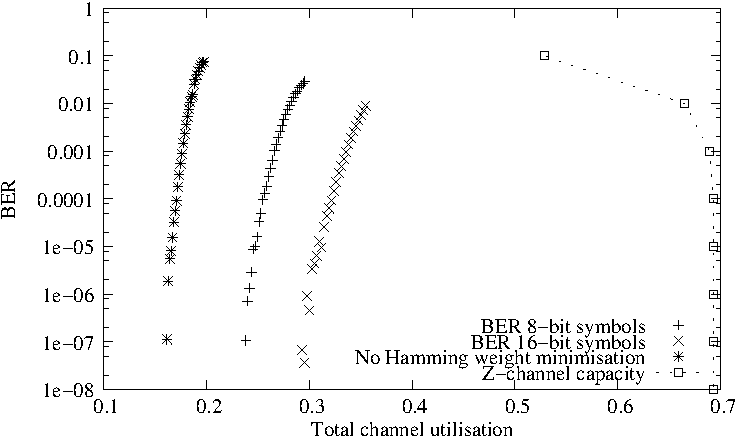
\includegraphics[width=0.8 \textwidth]{BERvsChannel} 
  \caption{Utilizacion del canal de 10 Gbps. Cada uno de los clientes (variando de 123 a 158) transmitieron 1 Gbit de datos. Notar la mejora en la utilización del ancho de banda comparada con~\cite{ortega11}.}
  \label{fig_use}
\end{figure}

En contraste con TDMA, en el esquema propuesto el atacante necesita interceptar cada una de las fibras ópticas para identificar cada usuario ya que son anonimizados luego de pasar por el hub central. Aun si el atacante puede identificar los datos, no podrá descifrarlos sin poseer la clave correcta al estar los datos desordenados por el time-hopping y normalizado el peso de Hamming.

\section{Estado del Arte}

Recordando que el objetivo es implementar un sistema de encriptación de fibra óptica a altas velocidades, se hará un repaso de las tecnologías disponibles actualmente para realizar esta tarea, así como las propuestas que apunten al mismo objetivo.

\subsection{Criptografía clásica}
Las comunicaciones ópticas pueden utilizar sin problemas algoritmos de criptografía clásicos tales como cifrado simétrico. La única dificultad consiste en que el procesamiento de datos debe ser lo suficientemente rápido para poder aplicarse al enlace de alta velocidad, lo que conlleva altos costos y procesadores con un alto consumo de energía, aunque la velocidad máxima de procesamiento puede reducirse arbitrariamente utilizando procesamiento en paralelo.

Actualmente, un dispositivo muy utilizado capaz de realizar criptografía a alta velocidad sobre fibra óptica es la FPGA, que con la correcta paralelización del procesamiento de datos, puede alcanzar la velocidad máxima permitida por sus tranceptores (por ejemplo, 400 Gbps~\cite{Algotronix}).

\subsection{Encriptación púramente óptica}
\label{optocry}
Otro método activamente investigado en la actualidad es la encriptación puramente óptica. La eliminación de la parte electrónica y la conversión a de los datos a señales eléctricas para procesamiento tiene muchas ventajas, principalmente en velocidad y potencia consumida por el sistema.
La dificultad principal en este método es en lograr el procesamiento y la implementación de los algoritmos necesarios solamente utilizando componentes ópticos. Actualmente este es un activo campo de investigación, ejemplos notables son los avances en la creación de compuertas lógicas puramente ópticas \cite{jung2008demonstration}, o la utilización de señales caóticas para transmisión~\cite{liu2002synchronized}.
La dificultad de implementación de estos métodos hace que actualmente estos sistemas estén en fase de desarrollo.

%High speed all-optical encryption and decryption using quantum dot semiconductor optical amplifiers 	http://www.tandfonline.com/doi/abs/10.1080/09500340.2013.856486#.VNHcKPtue00

\subsection{Encriptación cuántica}

\begin{figure}[t]
  \centering
  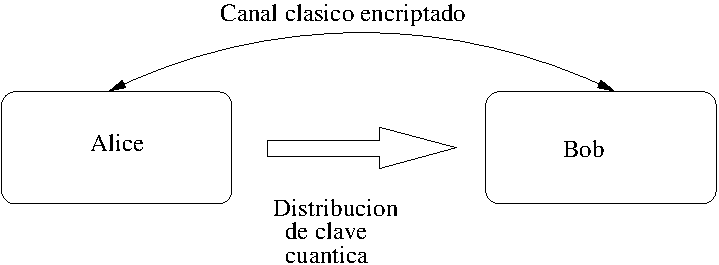
\includegraphics[width=0.7 \textwidth]{graphs/quantum} 
  \caption{Típico uso de distribución cuántica de claves. Notar que el canal cuántico es generalmente de menor velocidad que el clásico, ya que no se requiere de un grán ancho de banda para transferir las claves.}
  \label{fig_quant}
\end{figure}


\label{quantcry}
Una solución muy interesante a varios problemas criptográficos son las llamadas técnicas de encriptación cuántica, donde se aprovechan fenómenos físicos de mecánica cuántica para realizar varias tareas criptográficas.
Uno de los problemas criptográficos mas fácilmente resueltos utilizando mecánica cuántica es el de la distribución de claves, por lo que la distribución cuántica de claves (Quantum key distribution~\cite{grosshans2003quantum}) actualmente ya cuenta con muchas implementaciones comerciales e instalaciones a nivel metropolitano~\cite{sasaki2011field}. Generalmente se utilizan varios canales sobre una fibra óptica, unos llamados ``canales cuánticos'' utilizados solamente para la distribución de claves, y otros ``canales clásicos'' donde se utiliza criptografía clásica (ver esquema en la figura~\ref{fig_quant}).

Vale mencionar que la distribución segura de claves también puede realizarse en un canal clásico por medio de algoritmos matemáticos tales como Diffie-Hellman~\cite{diffie1976new} o bien la utilización de esquemas de clave pública.

Una posible ventaja de la criptografía cuántica es que al estar basado en fenómenos físicos comprobados, es imposible de atacar. Sin embargo, vulnerabilidades y fallas en la implementación afectan estos sistemas de la misma manera que afectan sistemas de criptografía clásicos~\cite{lydersen2010hacking}.


\subsection{Corrección de errores de canales asimétricos}

Una seccion importante de esta tesis es la descripción de una técnica de corrección de errores en canales asimétricos basada en el algoritmo de filtros de Bloom (ver~\ref{zbloom}). Recientemente surgió interés en campo de corrección de errores de canales asimétricos o unidireccionales, debido a la utilidad de estos algoritmos en sistemas de almacenamiento digitales\cite{tanakamaru201195}. Sin embargo, el número de artículos publicados acerca del tema sigue siendo muy reducido en comparación con las investigaciones de códigos de corrección para canales convencionales.

\subsection{Sistemas de comunicaciones ópticas}

Existen muchos esquemas tales como EPON~\cite{kramer2002ethernet} y sus derivados APON/BPON, utilizados por millones de usuarios en la actualidad.
Sin embargo, el sistema que mas se aproxima al descrito en esta tesis es el SPON (Secure Passive Optical Network). Existen muchos sistemas comerciales que proveen SPONs actualmente. Sistemas académicos se basan en encriptación puramente óptica tal como la descrita en \ref{optocry} (Ver~\cite{cincotti2009secure}). Algunas implementaciones proveen la misma funcionalidad que el sistema descrito en esta tesis, tale como~\cite{nadarajah2006implementation} aunque se diferencian en tipo de CDMA utilizado y la topología de la red óptica.
